\chapter{Software Design Specifications}
\newpage
\section{Définition}
Les Software Design Specifications (SDS), ou le cahier des charges de conception
du logiciel, à pour but de présenter l'architecture générale du logiciel.
La présentation se fait à deux échelles : à bas niveau avec des exemples de codes et
l'explication des bibliothèques utilisées. Et à un plus haut niveau avec des diagrammes
de fonctionnement, des exemples d'utilisations et des captures d'écran. À noter
que c'est dans cette section que nous traiterons des limites du logiciel. C'est
à dire tout ce que le logiciel ne sera pas en mesure de faire automatiquement.
Certaines recommandations vont donc être ennoncés, qu'il sera préférable de
respecter pour le bon fonctionnement de lockatme.
\section{Utilisation}
  \subsection{Installation Qualification}
Pour installer le logiciel lockatme, les utilisateurs auront deux options. Le
projet sera certainement upload sur pip. Il pourra donc utiliser la commande
suivante disponible sur toutes les distributions Linux, à condition d'avoir
installé le package pip de python :
\begin{lstlisting}[language=bash]
  ~$ pip install lockatme
\end{lstlisting}
Sinon il pourra tout simplement cloner le projet depuis GitHub en réalisant la
commande suivante :
\begin{lstlisting}[language=bash]
  ~$ git clone https://github.com/lockatme/lockatme-specifications.git
\end{lstlisting}
Le dossier comprendra un fichier exécutable en Python que l'utilisateur pourra
lancer avec la ligne suivante dans son shell :
\begin{lstlisting}[language=bash]
  ~$ python lockatme
\end{lstlisting}

  \subsection{Explication générale}
Une fois l'installation réalisée, comme expliqué dans la partie précédente,
le fichier exécutable \emph{lockatme.py} sera présent dans le dossier du logiciel. Son
exécution aura comme effet de verrouiller l'écran. Par défaut l'écran sera
recouvert d'un filtre transparent avec un cadenas (voir figure 4). A noter que
durant cette période de verrouillage, l'écran de l'ordinateur pourra très bien
se mettre en veille (écran noir), selon les configurations initiales de
l'utilisateur.
Pour sortir du verrouillage l'utilisateur aura juste à appuyer sur une touche
du clavier. Ensuite la reconnaissance faciale commencera immédiatement (voir
figure 5).
Un point rouge apparaissant et disparaissant indiquera une prise de
photo de la part de la webcam. Si une photo prise ainsi correspond à une photo
modèle, l'écran se déverrouillera. Au bout d'un moment (configurable dans le
fichier \emph{config.py}), si le déverrouillage échoue l'utilisateur sera invité à
entrer son mot de passe (voir figure 6).

  \subsection{Exemple sous i3}
    \subsubsection{Photos modèles}
Le choix des photos modèles devra se faire de manière autonome. À aucun moment
le logiciel invitera l'utilisateur à mettre des photos modèles dans le dossier
prévu cet effet. De même, pour le mot de passe devra être défini dans le
fichier \emph{password.py}. En cas d'absence de photos
modèles le logiciel demandera un mot de passe directement. Si le mot de passe
n'a pas été défini il suffira d'appuyer sur Entrée.
Voici la marche à suivre :
\begin{lstlisting}[language=bash]
  ~$ cp path/to/image ~/lockatme/images/
\end{lstlisting}
À noter qu'il est possible de mettre plusieurs photos modèles, dans la mesure
ou si l'image de la webcam correspond à l'une des photos le déverrouillage
fonctionnera.
\vspace{0.5cm}
Bien évidemment une image de bonne qualité est préférable, le logiciel ne
vérifiera pas la qualité de l'image. L'utilisateur devra donc voir à l'usage.

    \subsubsection{Raccourci clavier}
Cet exemple est réalisé à partir d'une distribution ArchLinux avec le Windows
manager i3. La marche à suivre est donc susceptible de changer.
\begin{lstlisting}[language=bash]
  ~$ cd .config/i3/
  ~/.config/i3/$ atom config
\end{lstlisting}
Exemple de config :
\fbox{\begin{minipage}{20em}
  program bindkey
  \\
  bindsym mod+o exec opera
  \\
  bindsym mod+g exec chromium
  \\
  bindsym mod+i exec spotify
  \\
  bindsym mod+p exec libreoffice
  \\
  bindsym mod+Shift+f exec firefox
  \\
\emph{bindsym mod+Key+binding exec lockatme}
\end{minipage}}

\newpage

    \subsubsection{Fermeture clapet}
Cette fonctionalité fait appel à l'Advanced Configuration and Power Interface
(acpi), qui sert aussi pour l'implémentation système. Nous y reviendrons donc
dans le VII.\\
La marche à suivre est la suivante :
\begin{lstlisting}[language=bash]
  ~$ cd /etc/
  /etc/$ mkdir acpi
  /etc/$ cd acpi
  /etc/acpi/$ mkdir events
  /etc/acpi/$ cd events
  /etc/acpi/events/$ atom lid
  /etc/acpi/events/$ cd ..
  /etc/acpi/$ atom lid.sh
\end{lstlisting}
Dans le dossier /etc/ il faut créer un dossier au nom de acpi. Ensuite à
l'intérieur de ce dernier créer un dossier events. Dans events il faut créer le
fichier \verb|lid| (voir ci dessous).\\
\\
\fbox{\begin{minipage}{15em}
event=button/lid LID close
\\
action=/etc/acpi/lid.sh "%e"
\end{minipage}}
\\
\\
Ce bout de code va permettre d'exécuter le fichier \verb|lid.sh| (voir ci dessous)
contenu dans \verb|/etc/acpi/|.\\
\\
\fbox{\begin{minipage}{15em}
lockatme
\end{minipage}}
\\
\\
Ainsi lorsque le clapet se fermera lockatme s'exécutera automatiquement.
\newpage

\section{Diagramme}
  \begin{figure}[h]
    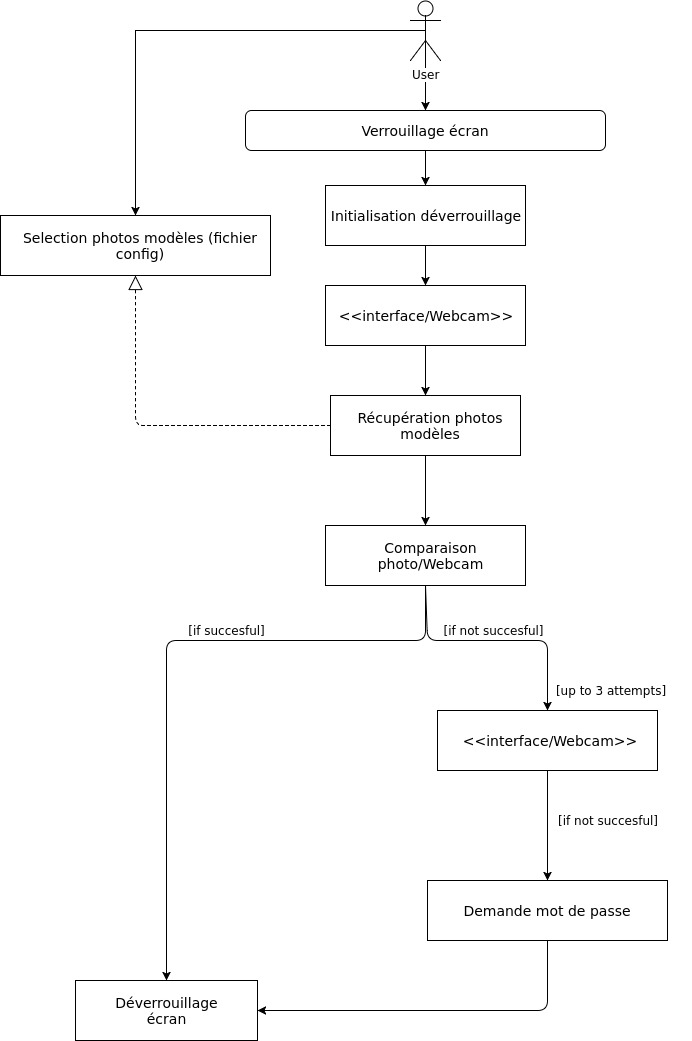
\includegraphics[width=0.75\linewidth]{Organisation}
    \caption{Diagramme explication du fonctionnenement général de lockatme}
  \end{figure}

\newpage

\section{Bibliothèques utilisées}
  \subsection{Contexte}
Lorsque nous avons commencé les recherches pour ce projet, nous nous sommes
d'abord penché sur l'utilisation de Open\_CV, un bibliothèque écrit en C/C++ qui
propose des bindings en Python. Open\_CV utilise le machine learning pour
reconnaître les visages au sein d'une image. La méthode de fonctionnement pour
identifier un visage dans une image est dit "en cascade". C'est à dire que le
programme va de manières successives et à différentes échelles, vérifier si
chaques parcelles de l'image ne contient pas un visage. Sans plus entrer dans
les détails, nous avons donc pu écrire quelques lignes de code qui nous
permettaient d'identifier les visages au sein d'une image (voir figure 8), mais aussi en direct
grâce à une webcam. Problème : cette option ne nous permettait pas de simplement
d'identifier une personne spécifique dans une image. Chose essentielle pour notre
logiciel.\\

\begin{figure}[h]
  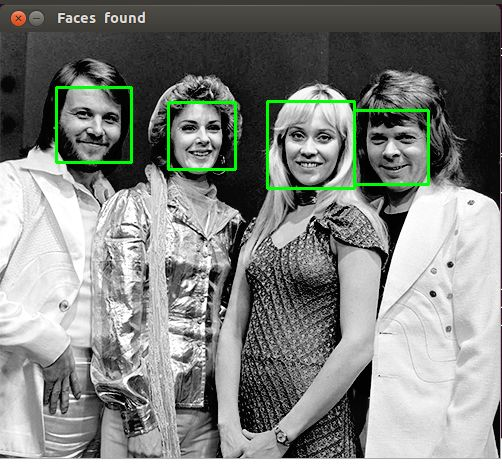
\includegraphics[width=0.8\linewidth]{face_open_cv}
  \caption{Reconnaissance visages avec programme bibliothèque Open\_CV}
\end{figure}

\newpage

Nous avons par la suite trouvé une autre bibliothèque bien plus avancé :
face\_recognition (https://github.com/ageitgey/face\_recognition). Avec celle-ci
les possibilités sont diverses, nous avons donc décidé d'utiliser face\_recognition
pour gérer la reconnaissance faciale de lockatme.

\subsection{Listing}
Lesquelles ? et Pourquoi ?
\\
  \begin{itemize}
    \item{Open\_CV : accès à la WebCam, nécessaire à la récupération de l'image
    WebCam}
    \item{face\_recognition : permet la reconnaissance facial spécifique par
    Machine learning}
  \end{itemize}

\subsection{Face\_recognition}
Face\_recognition est une bibliothèque très performante qui permet de détecter
les visages dans une image et d'identifier les protagonistes en fonction des
visages mémorisés (machine learning). La détection se fait grossièrement en
4 étapes :
\begin{itemize}
  \item{Trouver un visage dans l'image}
  \item{Analyser les caractéristiques faciales}
  \item{Comparer avec les visages connus}
  \item{Faire une prédiction sur la personne}
\end{itemize}

La technique de reconnaissance faciale est appelé Histogram of Oriented Gradients
(HOG). Tout d'abord les couleurs sont changés pour avoir une image en noir et blanc.
Ensuite l'idée est de regarder chaque pixel de l'image et de faire une flèche vers
le pixel adjacent le plus sombre. Chaque pixel est ainsi remplacé par une flèche
appelé gradient. Ce procédé permet d'avoir une représentation qui est indépendante
de la clareté ou de la sombreté de l'image. Mais une flèche par pixel rend
l'analyse trop pointue, ainsi l'image du début est séparée en carré de 16x16.
Dans chaque carré on trouve une flèche qui représente en moyenne la direction
la plus représenté des flèches de chaque pixel en son sein. Ainsi on a une
représentation globale et simple du visage (voir figure~\ref{fig:HOG})
\\
Pour reconnaître des personnes spécifiques, le logiciel ne va pas chercher à
comparer la représentation trouvé par HOG avec toutes les autres représentation
trouvé auparavant. Il va réaliser des mesures précises sur les visages trouvés
et ainsi émettre une décision par rapport aux mesures enregistrées dans le passé
sur d'autre image.
\\
\newpage
\begin{figure}[h]\label{fig:HOG}
  \begin{center}
  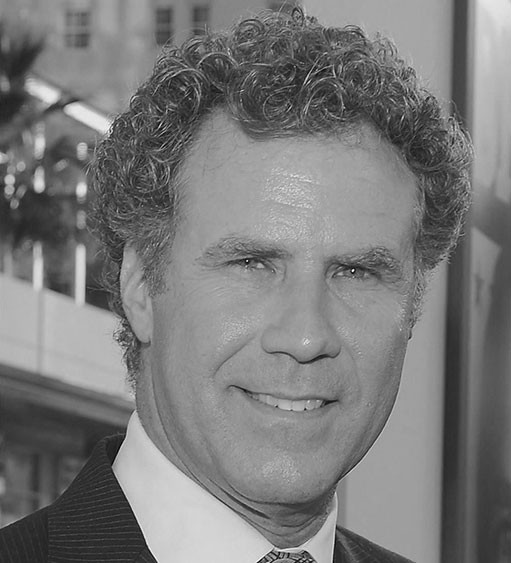
\includegraphics[width=0.4\linewidth]{HOG1}
  \caption{Exemple représentation HOG}
\end{center}
\end{figure}

\begin{figure}[h]\label{fig:HOG1}
  \begin{center}
  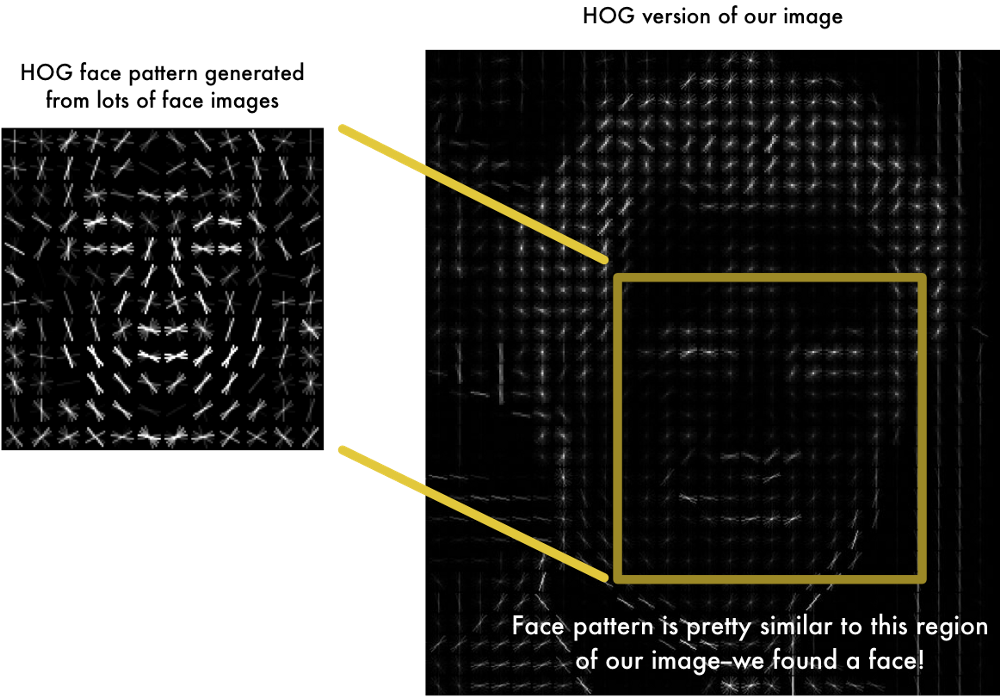
\includegraphics[width=0.7\linewidth]{HOG}
  \caption{Exemple représentation HOG}
\end{center}
\end{figure}
\newpage
\section{Exemple code}
Ci dessous le programme qui permet de passer en paramètre une image modèle et
une image à reconnaître. Le programme renvoit \verb|true| si la personne sur les deux
images est identique et \verb|false| sinon.
\\
\\
  \begin{verbatim}
import face\_recognition as fr


def is_recognized(imageSet, imagePath
    model_image = fr.load_image_file(imageSet
    unknown_image = fr.load_image_file(imagePath

    model_face_encoding = fr.face_encodings(model_image)[0
    unknown_face_encoding = fr.face_encodings(unknown_image)[0

    know_faces = [
        model_face_encoding
    ]

    results = fr.compare_faces(know_faces, unknown_face_encoding)

    return any(results)
  \end{verbatim}
Le programme va tout simplement prendre l'image modèle et "l'encoder"(HOG) et
la placer dans la liste des visages connus. L'autre image est également
encodé. L'avant dernière ligne permet de comparer les deux images encodées.
\\
\\
Sur le programme suivant même principe sauf que la reconnaissance se fait en direct
avec une Webcam. Le programme permet de dessiner un cadre rouge autour du/des
visages et de faire apparaître leur(s) nom(s) si il reconnait un visage.
L'encodage se fait ligne 9 et 10.\\
\\
\newpage
\begin{verbatim}
import facerecognition
import cv2

videocapture = cv2.VideoCapture(0)

jujuimage = facerecognition.loadimagefile("juju.jpg")
plimage = facerecognition.loadimagefile("pl.jpg")

jujufaceencoding = facerecognition.faceencodings(jujuimage)[0]
plfaceencoding = facerecognition.faceencodings(plimage)[0]

while True:
     ret, frame = videocapture.read()

     facelocations = facerecognition.facelocations(frame)
     faceencodings = facerecognition.faceencodings(frame, facelocations)

     for (top, right, bottom, left), faceencoding in zip(facelocations, faceencodings):
          #See if the face is a match for the known face(s)
          match = facerecognition.comparefaces([jujufaceencoding], faceencoding)
          match1 = facerecognition.comparefaces([plfaceencoding], faceencoding)

          name = "Unknown"
          if match[0]:
               name = "Juliette"
          if match1[0]:
              name = "PL"

          #Draw a box around the face
          cv2.rectangle(frame, (left, top), (right, bottom), (0, 0, 255), 2)

          #Draw a label with a name below the face
          cv2.rectangle(frame, (left, bottom - 35), (right, bottom), (0, 0, 255), cv2.FILLED)
          font = cv2.FONTHERSHEYDUPLEX
          cv2.putText(frame, name, (left + 6, bottom - 6), font, 1.0, (255, 255, 255), 1)

     #Display the resulting image
     cv2.imshow('Video', frame)

     #Hit 'q' on the keyboard to quit!
     if cv2.waitKey(1) & 0xFF == ord('q'):
          break

#Release handle to the webcam
videocapture.release()
cv2.destroyAllWindows()
\end{verbatim}
